\documentclass[11pt,a4paper]{article}
\usepackage[margin=2cm,top=1.5cm]{geometry}
\usepackage[T1]{fontenc}
\usepackage{lmodern}
\usepackage{amsmath,amssymb}
\usepackage{tikz}
\usepackage{array}
\usepackage{multicol}
\usepackage{enumitem}
\usepackage{titlesec}
\usepackage{needspace}
\setlength{\parindent}{0pt}
\setlength{\parskip}{4pt}
\titleformat{\section}{\Large\bfseries}{}{0pt}{}
\titlespacing*{\section}{0pt}{14pt}{8pt}

% Answer box: \ansbox{height}  (full width of current column)
\newcommand{\ansbox}[1]{%
  \par\noindent\begin{tikzpicture}
    \draw[line width=1.2pt] (0,0) rectangle (\linewidth-1.2pt,#1);
  \end{tikzpicture}\par\vspace{8pt}}

% Dotted writing lines: \writelines{n}
\newcommand{\writelines}[1]{%
  \par\foreach \i in {1,...,#1}{\vspace{14pt}\noindent\makebox[\linewidth]{\dotfill}\par}\vspace{6pt}}

\newcommand{\q}[1]{\par\needspace{4.8cm}\vspace{6pt}\textbf{#1.}~}

\begin{document}

\hfill Name: \underline{\hspace{5.5cm}} \quad Date: \underline{\hspace{3.5cm}}

\begin{center}
{\LARGE\bfseries Year 9 Algebra: End-of-Topic Assessment}
\end{center}

%==========================================================
\section*{Section A: Algebraic Expressions and Index Laws}

\q{1} Simplify by collecting like terms: $7c + 2d - 3c + 6d$
\ansbox{1.9cm}

\q{2} Simplify by collecting like terms: $6y^2 + 2y - 2y^2 - 7y$
\ansbox{1.9cm}

\q{3} Simplify using multiplication: $5r \times 2s$
\ansbox{1.9cm}

\q{4} Simplify using multiplication and index laws: $4y^2 \times 3y^6$
\ansbox{1.9cm}

\q{5} Simplify using division: $\dfrac{24n^8}{6n^3}$
\ansbox{1.9cm}

\q{6} Expand: $5(2t - 3)$
\ansbox{1.9cm}

\newpage
\q{7} Expand and simplify: $3(x + 2) + 4(2x - 5)$
\ansbox{3cm}

\q{8} Factorise completely: $15x + 20$
\ansbox{2.2cm}

\q{9} Factorise completely: $7p^2 - 21pq$
\ansbox{2.2cm}

%==========================================================
\section*{Section B: Substitution, Equations, and Inequalities}

\q{10} Given $a = 5$, $b = -2$, and $c = 4$, evaluate:

\begin{minipage}[t]{0.48\linewidth}
a) $3a - b$
\ansbox{2.5cm}
\end{minipage}\hfill
\begin{minipage}[t]{0.48\linewidth}
b) $c^2 + ab$
\ansbox{2.5cm}
\end{minipage}

\q{11} Solve the linear equation: $6x - 5 = 31$
\ansbox{3cm}

\q{12} Solve the linear equation: $4(3k + 2) = 44$
\ansbox{3cm}

\q{13} A plumber has a \$15 call-out fee and charges \$35 per hour on top of this.

\begin{minipage}[t]{0.48\linewidth}
a) Write an equation for the total cost, $C$, to hire him for $h$ hours.
\ansbox{2.5cm}
\end{minipage}\hfill
\begin{minipage}[t]{0.48\linewidth}
b) Use your equation to find how many hours the plumber worked if the total cost was \$190.
\ansbox{2.5cm}
\end{minipage}

\q{14} Solve the linear inequality: $5x + 2 \le 22$
\ansbox{2.5cm}

\q{15} Represent the solution from Question 14 on the number line below. Draw your circle and arrow clearly.

\vspace{1.2cm}
\begin{center}
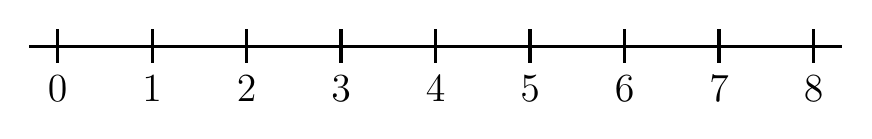
\begin{tikzpicture}[scale=1.2]
  \draw[line width=1.2pt] (-0.3,0) -- (8.3,0);
  \foreach \x in {0,...,8} {
    \draw[line width=1.2pt] (\x,0.18) -- (\x,-0.18);
    \node[below=7pt] at (\x,0) {\Large\x};
  }
\end{tikzpicture}
\end{center}

%==========================================================
\newpage
\section*{Section C: Linear Patterns and Graphs}

\q{16} A pattern of matchsticks grows as shown in the table below:

\vspace{4pt}
{\renewcommand{\arraystretch}{1.8}
\begin{tabular}{|p{3.4cm}|p{2.4cm}|p{2.4cm}|p{2.4cm}|p{2.4cm}|}
\hline
Pattern number ($n$) & 1 & 2 & 3 & 4 \\ \hline
Number of matches ($M$) & 5 & 9 & 13 & 17 \\ \hline
\end{tabular}}

a) Write a rule in words describing how the pattern grows.
\writelines{2}

b) Write an equation linking $M$ and $n$.
\ansbox{2cm}

c) Use your equation to predict the number of matches needed for Pattern 30.
\ansbox{2.5cm}

\q{17} Complete the table of values for the linear relationship $y = 3x + 1$:

\vspace{4pt}
{\renewcommand{\arraystretch}{1.8}
\begin{tabular}{|p{3.4cm}|p{2.4cm}|p{2.4cm}|p{2.4cm}|p{2.4cm}|}
\hline
$x$ & $-2$ & $-1$ & $0$ & $1$ \\ \hline
$y$ &  &  &  &  \\ \hline
\end{tabular}}

\needspace{12cm}\q{18} Plot the points from Question 17 on the coordinate grid below and draw a straight line through them across all four quadrants.

\begin{center}
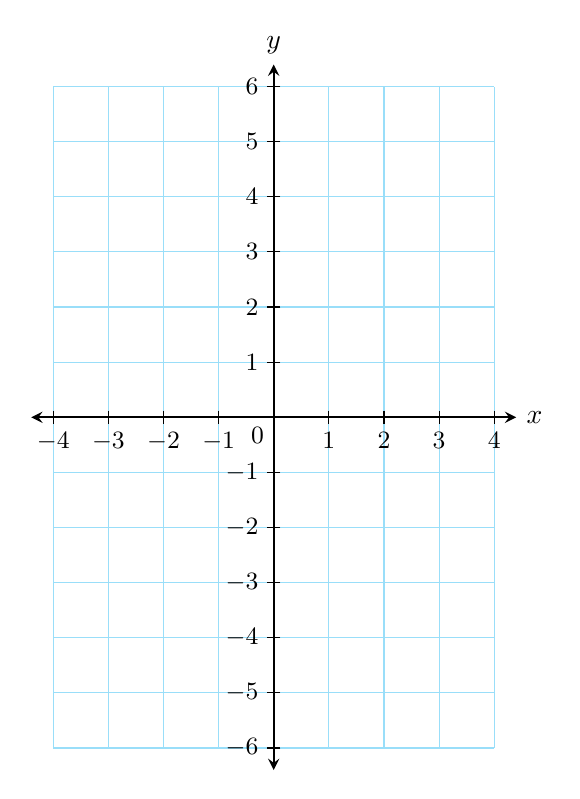
\begin{tikzpicture}[scale=0.7]
  \draw[cyan!40, thin] (-4,-6) grid (4,6);
  \draw[thick,<->,>=stealth] (-4.4,0) -- (4.4,0) node[right] {$x$};
  \draw[thick,<->,>=stealth] (0,-6.4) -- (0,6.4) node[above] {$y$};
  \foreach \x in {-4,-3,-2,-1,1,2,3,4} {
    \draw (\x,0.12) -- (\x,-0.12);
    \node[below, font=\small] at (\x,-0.1) {$\x$};
  }
  \foreach \y in {-6,...,-1,1,2,...,6} {
    \draw (0.12,\y) -- (-0.12,\y);
    \node[left, font=\small] at (-0.1,\y) {$\y$};
  }
  \node[below left, font=\small] at (0,0) {$0$};
\end{tikzpicture}
\end{center}

\q{19} For the line $y = -2x + 6$:

\begin{minipage}[t]{0.48\linewidth}
a) State the gradient ($m$) and state whether it is positive, negative, or zero.
\ansbox{2.5cm}
\end{minipage}\hfill
\begin{minipage}[t]{0.48\linewidth}
b) State the coordinates of the $y$-intercept.\\[\baselineskip]
\ansbox{2.5cm}
\end{minipage}

\newpage
\q{20} Two straight lines, Line A and Line B, are drawn on the grid below.

\begin{center}
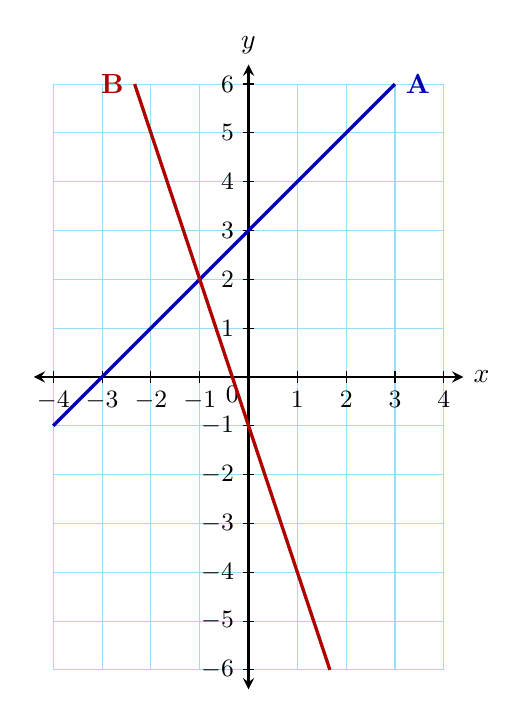
\begin{tikzpicture}[scale=0.62]
  \draw[cyan!40, thin] (-4,-6) grid (4,6);
  \draw[thick,<->,>=stealth] (-4.4,0) -- (4.4,0) node[right] {$x$};
  \draw[thick,<->,>=stealth] (0,-6.4) -- (0,6.4) node[above] {$y$};
  \foreach \x in {-4,-3,-2,-1,1,2,3,4} {
    \draw (\x,0.12) -- (\x,-0.12);
    \node[below, font=\small] at (\x,-0.1) {$\x$};
  }
  \foreach \y in {-6,...,-1,1,2,...,6} {
    \draw (0.12,\y) -- (-0.12,\y);
    \node[left, font=\small] at (-0.1,\y) {$\y$};
  }
  \node[below left, font=\small] at (0,0) {$0$};
  % Line A: y = x + 3
  \draw[very thick, blue!70!black] (-4,-1) -- (3,6) node[right] {\textbf{A}};
  % Line B: y = -3x - 1
  \draw[very thick, red!70!black] (-7/3,6) node[left] {\textbf{B}} -- (5/3,-6);
\end{tikzpicture}
\end{center}

a) Complete the table for each line.

\vspace{4pt}
{\renewcommand{\arraystretch}{2.2}
\begin{tabular}{|p{1.6cm}|p{3.2cm}|p{5.2cm}|p{3.6cm}|}
\hline
\textbf{Line} & \textbf{Gradient ($m$)} & \textbf{Direction (uphill or downhill from left to right)} & \textbf{$y$-intercept} \\ \hline
A & & & \\ \hline
B & & & \\ \hline
\end{tabular}}

b) Which line is steeper? Use the gradients to explain your answer.
\writelines{3}

\q{21} Jake says that $3x(2x + 1) = 6x^2 + 3x$. Lisa says that Jake is wrong and that expanding and equal are not the same.

Show, by substituting $x = 2$ and $x = -1$ into both expressions, that Jake is actually correct and both expressions are the same.

\begin{minipage}[t]{0.48\linewidth}
When $x = 2$:
\ansbox{4.5cm}
\end{minipage}\hfill
\begin{minipage}[t]{0.48\linewidth}
When $x = -1$:
\ansbox{4.5cm}
\end{minipage}

%==========================================================
\newpage
\section*{Marking grid}

\textbf{Cut scores}

3b 0--5 \quad 3P: 6--10 \quad 3A: 11--15 \quad 4B: 16--22 \quad 4P: 23--29 \quad 4A: 30--35 \quad 5b: 36--41 \quad 5P: 42--47 \quad 5A: 47--50

Award 2 marks for straightforward questions and 3 marks for questions involving several steps or reasoning. The maximum marks for each question are shown below.

\vspace{6pt}
{\renewcommand{\arraystretch}{1.6}
\begin{tabular}{|c|c|p{3cm}|c|c|p{3cm}|}
\hline
\textbf{Question} & \textbf{Max marks} & \textbf{Marks awarded} & \textbf{Question} & \textbf{Max marks} & \textbf{Marks awarded} \\ \hline
1 & 2 & & 12 & 3 & \\ \hline
2 & 2 & & 13 & 3 & \\ \hline
3 & 2 & & 14 & 2 & \\ \hline
4 & 2 & & 15 & 2 & \\ \hline
5 & 2 & & 16 & 3 & \\ \hline
6 & 2 & & 17 & 2 & \\ \hline
7 & 3 & & 18 & 3 & \\ \hline
8 & 2 & & 19 & 2 & \\ \hline
9 & 2 & & 20 & 3 & \\ \hline
10 & 3 & & 21 & 3 & \\ \hline
11 & 2 & & & & \\ \hline
\textbf{Total} & \textbf{50} & & & & \\ \hline
\end{tabular}}

%==========================================================
\newpage
\section*{Answers}

\begin{enumerate}[label=\textbf{\arabic*.}, leftmargin=*, itemsep=4pt]
\item $4c + 8d$
\item $4y^2 - 5y$
\item $10rs$
\item $12y^8$
\item $4n^5$
\item $10t - 15$
\item $3x + 6 + 8x - 20 = 11x - 14$
\item $5(3x + 4)$
\item $7p(p - 3q)$
\item a) $3(5) - (-2) = 15 + 2 = 17$ \\
      b) $4^2 + (5)(-2) = 16 - 10 = 6$
\item $6x = 36 \implies x = 6$
\item $12k + 8 = 44 \implies 12k = 36 \implies k = 3$ \quad (or $3k + 2 = 11 \implies k = 3$)
\item a) $C = 35h + 15$ \\
      b) $35h + 15 = 190 \implies 35h = 175 \implies h = 5$ hours
\item $5x \le 20 \implies x \le 4$
\item A solid (closed) circle at $4$ with an arrow pointing to the left along the number line.
\item a) Start with 5 matches and add 4 matches for each new pattern (or: multiply the pattern number by 4 and add 1). \\
      b) $M = 4n + 1$ \\
      c) $M = 4(30) + 1 = 120 + 1 = 121$ matches
\item When $x = -2$, $y = -5$; when $x = -1$, $y = -2$; when $x = 0$, $y = 1$; when $x = 1$, $y = 4$.
\item Points $(-2, -5)$, $(-1, -2)$, $(0, 1)$ and $(1, 4)$ plotted accurately, with a single straight line drawn through them and extended across the grid.
\item a) Gradient $m = -2$; it is negative. \\
      b) $(0, 6)$
\item a) Line A: gradient $m = 1$, uphill (positive), $y$-intercept $(0, 3)$. \\
      \phantom{a) }Line B: gradient $m = -3$, downhill (negative), $y$-intercept $(0, -1)$. \\
      b) Line B is steeper, because the size of its gradient (3) is greater than the size of Line A's gradient (1). The negative sign only tells us the direction, not the steepness.
\item When $x = 2$: $3(2)(2 \times 2 + 1) = 6 \times 5 = 30$ and $6(2)^2 + 3(2) = 24 + 6 = 30$. \\
      When $x = -1$: $3(-1)(2 \times (-1) + 1) = (-3)(-1) = 3$ and $6(-1)^2 + 3(-1) = 6 - 3 = 3$. \\
      Both expressions give the same value each time, so Jake is correct: expanding gives an equivalent (equal) expression.
\end{enumerate}

\end{document}
